


%%%%%%%%%%%%%%%%
%%  Introduction
%%%%%%%%%%%%%%%%


%% Contents
%
%    - General considerations on Complex Systems, positioning etc (thesis in cs science etc)
%    - Thematic introduction, geographical introduction of the subject.
%
%   - precisions on v1 memoire : foreword ?
%
%    - reading precisions : organisation, interdependances etc 
%
%   - reflexive aspect : here ?  


%\chapter*{Introduction}{Introduction}
\chapter*{Introduction}


% to have header for non-numbered introduction
\markboth{Introduction}{Introduction}


% -- citations on hold --
%\headercit{\bpar{It's when you shuffle the anthill that you get a touch of all its complexity.}{C'est quand on donne un coup de pied dans la fourmilière qu'on se rend compte de toute sa complexité.\comment[AB]{je persiste a dire que c'est oas une tres bonne idee !}\comment[FL]{Incipit de son directeur de these est maladroit}}
%}{Arnaud Banos}{}



\bigskip




%\bpar{
%``In consequence of a technical issue, traffic is interrupted on the line B of RER, for an unknown duration. More information will be given as soon as available''. There is a high probability that someone having lived or spent some time in the metropolitan region of Paris has already heard this frightening announce and endured the difficult consequences the rest of his day. But he might not be aware of the ramifications of causal cascades induced by this not-so-rare event. Territorial Systems, whatever the layers considered in their definitions, will always be extremely complex and interrelations at numerous temporal and spatial scales participate in the emergent behaviors observed at any levels of the system. Martin is a student who daily commutes from Paris to Palaiseau and will miss today a crucial exam, what will have a profound impact on his professional life : implications at a long time scale, small spatial scale and agent granularity. Yuangsi is connecting Orly and Roissy Airports, in his trip from London to Beijing, will miss his plane and his sister's wedding : large spatial scale, short time scale, agent granularity. A collective petition emerges from users, leading to new social organizational patterns and reaction from transportation authority that results in efforts to increase levels of service : mesoscopic temporal and spatial scale, swarm of agents granularity. Looking for causes of the event will also lead to intricate processes at various scales, none of which seems to be a better explication than others : historical railway network in Parisian region shaped further extensions and RER B followed the former \textit{Ligne de Sceaux}, \noun{Delouvrier}'s schema for regional development, and its subsequent partial execution, are elements of explanation of structural weaknesses of Parisian public transportation network~\citep{gleyze2005vulnerabilite}; commuting patterns consequent to territorial organisation induce an overload of particular lines and thus a necessary increase in exploitation incidents. 
%}{
%``En conséquence d'un problème technique, le trafic est interrompu sur la ligne B du RER pour une durée indéterminée. Plus d'information seront fournies dès que possible''. Il y a des fortes chances pour que quiconque ayant vécu ou passé un peu de temps en région parisienne ait déjà entendu cette annonce glaçante et en ait subi les conséquences pour le reste de la journée. Mais il ne se doute sûrement pas des ramifications des cascades causales induites par cet évènement presque banal. Les systèmes territoriaux, quelles que soient les aspects considérés pour leur définition, ont une complexité croissante lorsqu'on augmente leur nombre, les interrelations à de nombreuses échelles spatiales et temporelles participant à la production des comportements émergents observés à tout niveau du système. Martin est un étudiant qui fait l'aller-retour journalier entre Paris et Palaiseau and manquera un examen crucial, ce qui aura un impact profond sur sa vie professionnelle : implications à une longue échelle de temps, une petite échelle spatiale et à la granularité de l'agent. Yuangxi était en train de relier les aéroports d'Orly et Roissy dans son voyage de Londres à Pékin et va manquer son avion ainsi que le mariage de sa soeur : grande échelle spatiale, courte échelle temporelle, granularité de l'agent. Une pétition collective émerge des voyageurs, conduisant à la création d'une organisation qui mettra la pression sur les autorités pour qu'elles augmentent le niveau de service : échelle temporelle et spatiales mesoscopique, granularité de l'aggregation d'agents.
%\comment[FL]{encore une fois : l'exemple mobilite quotidienne pour commencer me semble mal choisi}
%La recherche de cause possible à l'incident conduira à des processus intriqués à diverses échelles, parmi lesquels aucun ne semble être une meilleure explication ; le développement historique du réseau ferroviaire en région parisienne a conditionné les évolutions futures et le RER B a suivi l'ancienne Ligne de Sceaux, le plan de \noun{Delouvrier} pour le développement régional et son execution partielle, sont également des éléments d'explication de la structure du réseau parisien de transports en commun qui conditionne la perturbation~\cite{gleyze2005vulnerabilite} ; les motifs pendulaires dus à l'organisation territoriale induisent une surcharge de certaines ligne et ainsi nécessairement une augmentation des incidents d'exploitation.

%}


\bpar{
\textit{Would the fog machine on the Saclay plateau be the only atemporal artefact in this metropolitan environment still searching for its own identity? Let's project us in 2100, in this southern suburb of what will still be Paris. Local transformations have indeed happened, but not in the expected way, the local climate being still fond of this well-known fog. However, the urban environment and the relation to the city are entirely conditioned by a proximity to structural transportation lines: the disappearance of fossil fuel transportation modes, then of all light vehicles through the technological failure of electric alternatives, have exacerbated the role of existing train or metro lines. Densities have progressively increased around stations to produce impressing tower compounds, whereas the peri-urban space became progressively empty. Concerning transportation infrastructures, they stayed quite at the identical after 2030, the few available resources being dedicated to their maintenance, and their extension became conjointly rapidly out of the political agendas. This plateau is therefore filled with abandoned buildings, since it still expects this line of the Grand Paris Express which finally would never have been realized. Nature progressively finds its way again.}
}{
\textit{La machine à brouillard du Plateau de Saclay serait-elle le seul artefact intemporel dans cet environnement métropolitain qui se cherche toujours ? Projetons nous en 2100, dans cette banlieue sud de ce qui sera toujours Paris. Les bouleversements locaux ont bien eu lieu, mais pas de la façon attendue, le climat local étant toujours féru de ce fameux brouillard. Par contre, l'environnement urbain et la relation à la ville sont entièrement conditionnés par une grande proximité aux lignes de transport lourd : la disparition des moyens de transport thermiques, puis de l'ensemble des véhicules légers par échec technologiques des alternatives électriques, ont exacerbé le rôle des lignes de train ou de metro existantes. Les densités ont progressivement augmenté autour des gares pour produire d'impressionnants complexes de tours, tandis que les espaces péri-urbains se vidaient progressivement. Les infrastructures de transport sont quant à elles restées quasiment à l'identique après 2030, le peu de ressources disponibles étant dédié à leur entretien, et leur extension étant conjointement sortie rapidement des agendas politiques. Ce plateau est alors rempli de bâtiments à l'abandon, puisqu'il attend toujours ce tronçon du Grand Paris Express qui n'aura finalement jamais été réalisé. La nature reprend peu à peu ses droits.}
}


\bpar{
This scenario for a low budget anticipation film has the advantage of revealing the existence of complex processes entangled at different space and time scales in the production of cities: the historical development of the railway network in the Parisian region conditioned the future evolutions, the RER B followed the old Ligne de Sceaux; the masterplan by \noun{Delouvrier} for regional development and its incomplete realization are elements explaining the structure of the Parisian public transportation network which strongly condition urban development in our scenario; relocation processes within the metropolitan space, related to a more or less strong need for proximity or accessibility depending on transportation modes used, play they role in the urban evolution; in the case of the plateau of Saclay specific planning processes at different levels play a crucial role in the differentiation of the territory.
}{
Ce pitch pour film d'anticipation à petit budget a pour avantage de nous révéler l'existence de processus complexes intriqués à différentes échelles de temps et d'espace dans la fabrique des villes : le développement historique du réseau ferroviaire en région parisienne a conditionné les évolutions futures, le RER B a suivi l'ancienne Ligne de Sceaux ; le plan de \noun{Delouvrier} pour le développement régional et son execution partielle sont des éléments d'explication de la structure du réseau parisien de transports en commun qui conditionnent fortement le développement urbain dans notre scenario ; les processus de relocalisation au sein de l'espace de la métropole, liés à une plus ou moins grande nécessité de proximité ou d'accessibilité selon les modes de transports utilisés, participent à l'évolution urbaine ; dans le cas du plateau de Saclay des processus de planification spécifiques à différents niveaux jouent un rôle crucial dans la différentiation du territoire.
}



\bpar{
The list could be much further developed, since each approach brings its mature vision related to a scientific body of knowledge in different disciplines such as geography, urban economics, transportation. This anticipation scenario is enough to give a glance on the complexity of territorial systems we will study. Our aim here is to dive within this complexity, and more particularly to give an original viewpoint on the study of relations between transportation networks and territories. The choice of this positioning will be largely discussed in a thematic part, and we now concentrate on the originality of the point of view we will take.
}{
La liste pourrait être ainsi continuée indéfiniment, chaque approche apportant sa vision mature correspondant à un corpus de connaissances scientifiques dans des disciplines diverses comme la géographie, l'économie urbaine, les transports. Ce scénario d'anticipation est suffisant pour faire ressentir la complexité des systèmes territoriaux que nous étudierons. Notre but ici est de se plonger dans cette complexité, et en particulier de donner un point de vue original sur l'étude des relations entre réseaux de transport et territoires. Le choix de cette position sera largement discuté dans une partie thématique, et nous nous concentrons à présent sur l'originalité du point de vue que nous allons prendre.
}





\section*{On General Positioning}{De la position générale}


\bpar{
\emph{The ambition of this thesis is to have no a priori ambition.} Such an introduction, although seeming rash, contains at all levels the implicit logics behind our research process. At the first degree, we try as much as possible to take a exploratory and constructive approach, as much on theoretical and methodological domains than thematic domain, but also proto-methodological (tools applying the method) : if unidimensional or integrated ambitions should emerge, they would be conditioned by the arbitrary choice of a time sampling among the continuity of the dynamic that structures any research project. In the structural sense, the self-reference that underlines an apparent contradiction points out the central aspect of reflexivity in our constructive approach, as much in the sense of the recursion of theoretical apparels, than for application of tools and methods developed to the work itself, or in the sense of the co-construction of the different approaches and of the different thematic axis. The processus of knowledge production can this way be understood as a metaphor of studied processes. Finally, from a point of view closer to the interpretation, it suggests the intention of a delicate positioning linking a political positioning which necessity is intrinsic to humanities (for example here against the technocratic application of models, or for the development of tools for an Open Science) with a rigor of objectivity coming more from other fields used, position that impose an increased prudence.
}{
\emph{L'ambition de cette thèse est de ne pas avoir d'ambition a priori.}
 Cette entrée en matière, rude en apparence, contient à différents niveaux les logiques sous-jacentes à notre processus de recherche. Au sens propre, nous nous plaçons tant que possible dans une démarche constructive et exploratoire, autant sur les plans théorique et méthodologique que thématique, mais encore proto-méthodologique (outils appliquant la méthode) : si des ambitions unidimensionnelles ou intégrées devaient émerger, elles seraient conditionnées par l'arbitraire choix d'un échantillon temporel parmi la continuité de la dynamique qui structure tout projet de recherche. Au sens structurel, l'auto-référence qui soulève une contradiction apparente met en exergue l'aspect central de la réflexivité dans notre démarche constructive, autant au sens de la récursivité des appareils théoriques, de celui de l'application des outils et méthodes développés au travail lui-même ou que de celui de la co-construction des différentes approches et des différents axes thématiques. Le processus de production de connaissance pourra ainsi être lu comme une métaphore des processus étudiés. Enfin, sur un plan plus enclin à l'interprétation, cela suggérera la volonté d'une position délicate liant une conscience politique dont la nécessité est intrinsèque aux sciences humaines (par exemple ici contre l'application technocratique des modèles, ou pour le développement d'outils luttant pour une science ouverte) à une rigueur d'objectivité plus propre aux autres champs abordés, position forçant à une prudence accrue.
}

%\comment[AB]{Déclaration discutable : si j’ai bien compris l’argumentaire, ton absence d’ambition tient 1) à l’absence de quête d’universalité (dépendance au contexte) et 2) à la dimension politique inhérente à ton objet. Je te ferais dire que 1) l’absence d’universalité n’est pas une tare (c’est même la norme en SHS) et 2) la dissociation science/politique ne tient plus la route depuis bien longtemps et ne concerne qu’un micro domaine des sciences les plus abstraites et théoriques (maths fondamentales, physique théorique peut-être,…what else ?)}[rq : logique proche de Morin - but contenu dans moyen ? - endogene.]



\section*{Scientific context : paradigms of complexity}{Contexte scientifique : paradigmes de la complexité}


% \footnote{pour lesquels il n'existe pas de définition unifiée mais dont les champs d'application couvrent une étendue allant des neurosciences à la finance quantitative, en passant par exemple par la sociologie quantitative, la géographie quantitative, la biologie intégrative, etc.~\cite{newman2011complex}, et pour l'étude desquels diverses approches complémentaires peuvent être appliquées, comme les Systèmes Dynamiques, la Modélisation Basée Agent, la Théorie des Matrices Aléatoires}


\bpar{
To better introduce our subject, it is necessary to develop the scientific context we will be integrated into. This context is crucial both to understand the general epistemology underlying research questions, and to be aware of the variety of methods and tools used.
}{
Pour une meilleure introduction du sujet, il est nécessaire d'insister sur le cadre scientifique dans lequel nous nous positionnons. Ce contexte est crucial à la fois pour comprendre les concepts épistémologiques implicites dans nos questions de recherche, et aussi pour être conscient de la variété de méthodes et outils utilisés.
}


\bpar{
Contemporaneous science is progressively taking the shift of complexity in many fields that we will illustrate in the following, what implies an epistemological mutation to abandon strict reductionism\footnote{In a schematic way, reductionism consists in the epistemological positioning that systems are entirely understandable from the fundamental elements they are constituted of and from the laws driving their evolution. Superior levels have neither an autonomy nor irreducible causal powers.} that failed in most of its synthesis attempts~\cite{anderson1972more}. \cite{arthur2015complexity} recently recalled that a mutation of methods and paradigms was also at stake, through the increasing role of computational approaches replacing purely analytical techniques generally limited in their modeling and resolution scope. Capturing \emph{emergent properties} in models of complex systems is one of the ways to understand the essence of these approaches.
}{
La science contemporaine prend progressivement le tournant de la complexité dans de nombreux champs que nous illustrerons par la suite, ce qui implique une mutation épistémologique pour abandonner le réductionnisme\footnote{De manière schématique, le réductionnisme consiste en la position épistémologique que les systèmes sont entièrement compréhensibles à partir des éléments fondamentaux les constituant et des lois régissant leur évolution. Les niveaux supérieurs n'ont ni autonomie ni pouvoirs causaux irréductibles.} strict qui a échoué dans la majorité de ses tentatives de synthèse~\cite{anderson1972more}. \cite{arthur2015complexity} a rappelé récemment qu'une mutation des méthodes et paradigmes en était également un enjeu, par la place grandissante prise par les approches computationnelles qui remplacent les résolutions purement analytiques généralement limitées en possibilités de modélisation et de résolution. La capture des \emph{propriétés émergentes} par des modèles de systèmes complexes est une des façons d'interpréter la philosophie de ces approaches.
}



\bpar{
These considerations are well known in Social Sciences and Humanities (both quantitative and qualitative), for which the complexity of studied agents and systems is one of the justifications of their existence: if humans were indeed particles, we could expect that most fields studying them would have never emerged, as thermodynamics would have solved most of social issues. \footnote{Even if this affirmation can also be discussed, since classical physics also failed in their attempts to include irreversibility and evolutions of Complex Adaptive Systems as \cite{prigogine1997end} points out.}. They are however less known nor accepted in more ``hard'' sciences such as physics: \cite{laughlin2006different} develops a view of physics at a similar position of a ``frontier of knowledge'' compared to other more recent fields that could appear as being still in their genesis. Most of knowledge concerns classical simple structures, whereas a large number of systems appear as \emph{self-organized}, in the sense that the single microscopic laws are not enough to determine macroscopic properties unless system evolution is entirely simulated (more precisely this view can be taken as a definition of emergence on which we will come back later, and self-organized properties are indeed emergent). This corresponds to the first nightmare of Laplace's Deamon developed in~\cite{deffuant2015visions}.
}{
Ces considérations sont bien connues des Sciences Humaines et Sociales (qualitatives et quantitatives) pour lesquelles la complexité des agents et systèmes étudiés est une des justifications de leur existence : si les humains étaient effectivement des particules, on pourrait s'attendre à ce que la majorité des disciplines les prenant comme objet d'étude n'aient jamais émergé puisque la thermodynamique aurait alors résolu la majorité des problèmes sociaux\footnote{Bien que cette affirmation soit elle-même discutable, les sciences physiques classiques ayant également échoué à prendre en compte l'irréversibilité et l'évolution de systèmes complexes adaptatifs comme le soulignent~\cite{prigogine1997end}.}. Elles sont au contraire moins connues et acceptées en sciences ``dures'' comme la physique : \cite{laughlin2006different} développe une vision de la physique à la même position de ``frontière des connaissances'' que d'autres champs plus récents qui pourraient sembler en être encore à leur genèse. La plupart des connaissances actuelles concernent des structures classiques simples, alors qu'un grand nombre de systèmes présentent des propriétés \emph{d'auto-organisation}, au sens où les lois microscopiques ne sont pas suffisantes pour inférer les propriétés macroscopiques du système à moins que son évolution ne soit entièrement simulée (plus précisément cette vision peut être prise comme une définition de l'émergence sur laquelle nous reviendrons par la suite, or des propriétés auto-organisées sont par nature émergentes). Cela correspond au premier cauchemar du Démon de Laplace développé dans~\cite{deffuant2015visions}. 
} 


%-------------------------------------------------



\bpar{
At the crossroads of epistemological positions, methods, and fields of applications, sciences of \emph{Complexity} focus on the importance of emergence and self-organization in most of phenomena of the real world, which make it lie closer to a frontier of knowledge closer than we can imagine for classical disciplines \cite{laughlin2006different}. These concepts are indeed not recent and had already been shown by~\cite{anderson1972more}. We can also interpret Cybernetics as a precursor of Complexity Sciences, by reading it as a bridge between technology and cognitive sciences~\cite{wiener1948cybernetics}, and moreover by developing the notions of feedback and control.
}{
A la croisée de positionnements épistémologiques, de méthodes et de champs d'application, les \emph{Sciences de la complexité} se concentrent sur l'importance de l'émergence et de l'auto-organisation dans la plupart des phénomènes réel, ce qui les place plus proche de la frontière des connaissances que ce que l'on peut penser pour des disciplines classiques \cite{laughlin2006different}. Ces concepts ne sont pas récents et avaient déjà été mis en valeur par~\cite{anderson1972more}. On peut aussi interpréter la Cybernétique comme un précurseur des Sciences de la Complexité en la lisant comme un pont entre technologie et sciences cognitives~\cite{wiener1948cybernetics}, et surtout en développant les notions de rétroaction et de contrôle.
}

\bpar{
Later, Synergetics~\cite{haken1980synergetics} paved the way for a theoretical approach of collective phenomena in physics. Possible reasons for the recent growth of works claiming a complexity approach are numerous. The explosion of computing power is surely one of these because of the central role of numerical simulations~\cite{varenne2010simulations}. They could also be related to epistemological progresses: introduction of the notion of perspectivism~\cite{giere2010scientific}, finer reflexions around the nature of models~\cite{varenne2013modeliser}\footnote{In that frame scientific and epistemological progresses can not be dissociated and can be seen as co-evolving, in the sense of a strong interdependency and a mutual adaptation}.
}{
Plus tard, la Synergétique~\cite{haken1980synergetics} a posé les bases d'approches théoriques des phénomènes collectifs en physique. Les causes possibles de la croissance récente du nombre de travaux se réclamant d'approches complexes sont nombreuses. L'explosion de la puissance de calcul en est certainement une vu le rôle central que jouent les simulations numériques~\cite{varenne2010simulations}. Elles peuvent aussi être à chercher auprès de progrès en épistémologie : introduction de la notion de perspectivisme~\cite{giere2010scientific}, reflexions plus fine autour de la nature des modèles~\cite{varenne2013modeliser}\footnote{Dans ce cadre, les progrès scientifiques et épistémologiques ne peuvent pas être dissociés et peuvent être vus comme étant en co-évolution, au sens d'une forte interdépendance et d'une adaptation mutuelle.}.
}

\bpar{
The theoretical and empirical potentialities of such approaches play surely a role in their success\footnote{Although the adoption of new scientific practices may be strongly biased by imitation and lack of originality~\cite{dirk1999measure}, or in a more ambivalent way, by marketing strategies independent of knowledge strategies, as the fight for funds is becoming a huge obstacle for research~\cite{bollen2014funding}.}, as confirmed by the various domains of application (see~\cite{newman2011complex} for a general survey), as for example Network Science~\cite{barabasi2002linked}; Neuroscience~\cite{koch1999complexity}; Social Sciences including Geography~\cite{manson2001simplifying,pumain1997pour}; Finance with econophysics approaches~\cite{stanley1999econophysics}; Ecology~\cite{grimm2005pattern}. The Complex Systems Roadmap~\cite{2009arXiv0907.2221B} proposes a double entry to studies on Complex Systems: an horizontal approach connecting fields of study with transversal questions on theoretical foundations of complexity and empirical common stylized facts, and a vertical approach to disciplines, with the aim at constructing integrated disciplines and corresponding multi-scale heterogeneous models. Interdisciplinarity is thus central in our scientific background.
}{
Les potentialités théoriques et empiriques de telles approchent jouent nécessairement un rôle dans leur succès\footnote{Même si l'adoption de nouvelles pratiques scientifiques peut par ailleurs être biaisé par l'imitation et le manque d'originalité~\cite{dirk1999measure}, ou de façon plus ambivalente, par des stratégies de positionnement indépendante des stratégies de connaissance, puisque le combat pour les fonds est un obstacle croissant à une recherche saine~\cite{bollen2014funding}.}, comme le confirme les domaines très variés d'application (voir~\cite{newman2011complex} pour une revue très générale), comme par exemple la Science des Réseaux~\cite{barabasi2002linked}; les Neurosciences~\cite{koch1999complexity}; les Sciences Humaines et Sociales,  dont la Géographie~\cite{manson2001simplifying,pumain1997pour}; la Finance avec les approches éconophysiques~\cite{stanley1999econophysics}; l'Ecologie~\cite{grimm2005pattern}. La Feuille de Route des Systèmes Complexes~\cite{2009arXiv0907.2221B} propose une double lecture des travaux en Complexité: une approche horizontale faisant la connexion entre champs d'étude par des questions transversales sur les fondations théoriques de la complexité et des faits stylisés empiriques communs, et une approche verticale, dans le but de construire des disciplines intégrées et les modèles multi-scalaires hétérogènes correspondants. L'interdisciplinarité est ainsi cruciale pour notre contexte scientifique.
}


\section*{Interdisciplinarity}{Interdisciplinarité}



\bpar{
We must further insist on the role of interdisciplinarity in the research positioning taken here. This is as much a work in Theoretical and Quantitative Geography than in Complex Systems Modeling, being finally both depending on the point of view taken by the reader. In that sense, we claim it to belong to \emph{Complex Systems Science} that we aim at positioning as a proper discipline through this precise implementation\footnote{An abstract level of reading of the work in its entirety will bring informations on knowledge production itself, as we will develop in~\ref{sec:knowledgeframework}.}. There are risks of being read with mistrust or even defiance by scholars of various concerned disciplines, as recent examples of misunderstandings and conflicts have illustrated~\cite{dupuy2015sciences}. We need to recall the importance of \noun{Banos}' virtuous circle between disciplinarity and interdisciplinarity~\cite{banos2013pour}. It must necessarily imply different scientific agents, and it is complicated for an agent to be positioned in the two branches; our scientific background will have to allow us to not be positioned only within \emph{geographical disciplinarity} (even if it will simultaneously be a crucial component) but as much within Complex Systems (which is interdisciplinary, see~\ref{sec:epistemology} to go beyond the apparent contradiction), and our scientific and epistemological sensitivity leads us to do the same.
}{
Il est important d'insister sur le rôle de l'interdisciplinarité dans la position de recherche prise ici. Il s'agit autant d'un travail en Géographie Théorique et Quantitative qu'en Modélisation de Systèmes Complexes, étant finalement les deux à la fois selon le point de vue que prendra le lecteur. En ce sens, nous le réclamons de la \emph{Science des Systèmes Complexes} que nous tenterons de positionner comme discipline propre à travers cette implémentation précise\footnote{Un niveau de lecture abstrait du travail dans son ensemble apportera des informations sur la production de connaissance elle-même, comme nous le développerons en~\ref{sec:knowledgeframework}.}. Ce n'est pas sans risques d'être lu avec méfiance voir défiance par les tenants des disciplines classiques, comme des exemples récents de malentendus ou conflits ont récemment illustré~\cite{dupuy2015sciences}. Il faut se rappeler l'importance de la spirale vertueuse de \noun{Banos} entre disciplinarité et interdisciplinarité~\cite{banos2013pour}. Celle-ci doit nécessairement impliquer différents agents scientifiques, et il est compliqué pour un agent de se positionner dans les deux branches ; notre fond scientifique devra nous permettre de ne pas de nous positionner uniquement dans la \emph{disciplinarité géographique} (même si celle-ci sera simultanément une composante cruciale) mais bien aussi dans celle des Systèmes Complexes (qui est interdisciplinaire, voir~\ref{sec:epistemology} pour contourner la contradiction apparente), et notre sensibilité scientifique et épistémologique nous pousse à faire de même.
}

% rq : point de vue = grille de lecture
% \comment[AB]{je trouve que tu abandonnes bien vite la partie. Pourquoi renoncer dès le début alors que tu pourrais laisser la liberté à celui/celle qui te lit de décider si c’est AUSSI de la géo ou non ?}


% -- inutile --
%\bpar{
%The positioning of \noun{Batty} proposing \textit{A new Science of Cities}~\cite{batty2013new} (that he subtly presents as \textit{The} new science of cities) is directed towards an integration of disciplines and methods into a science defined by its object of study, cities.
%Its theoretical and epistemological weaknesses (no theoretical constructions of studied geographical objects on the one hand, approximative contextualization of complexity) combined with an overall impression of \emph{pot-pourri} of forgotten works
% (space syntax, land-use models), unfortunately avoid us to use it as we will use geographical theories (e.g. evolutive urban theory) in an appropriated epistemological complexity context. Yet our reading of this work may be the result of a misunderstanding due to different cultural backgrounds.
%}
%{
%Le positionnement de \noun{Batty} lorsqu'il propose \textit{Une Nouvelle Science des Villes}~\cite{batty2013new} %(qu'il présente avec humour comme \textit{La} nouvelle science des villes)
%, se présente comme une intégration des disciplines et méthodes vers une science définie par son objet d'étude, les villes.
%Its theoretical and epistemological weaknesses (no theoretical constructions of studied geographical objects on the one hand, approximative contextualization of complexity) combined with an overall impression of \emph{pot-pourri} of forgotten works (space syntax, land-use models), unfortunately avoid us to use it as we will use geographical theories (e.g. evolutive urban theory) in an appropriated epistemological complexity context.  Yet our reading of this work may be the result of a misunderstanding due to different cultural backgrounds. \comment[Arnaud]{j'espère que tu abuses ? :) !! Argument d'autorité}[yes, changer positionnement complètement malvenu] \comment[Florent]{attention arguments autorité ; insister sur difficulté à intégrer paradigmes plutot que juger précédents}[idem]
%}




\bpar{
The scientific evolution of complexity sciences, that some see as a revolution~\cite{colander2003complexity}, or even as \emph{a new kind of science}~\cite{wolfram2002new}, could indeed face intrinsic difficulties due to behaviors and a-priori of researchers as human beings. More precisely, the need for interdisciplinarity which makes the strength of Complexity Science may be one of its greatest weaknesses, since the highly partitioned structure of the organization of science may have negative impacts on works involving different disciplines. We do not tackle the issue of over-publication, quantification, competition, which is more linked to a question of Open Science and its ethics, also of high importance but of an other nature. That barrier haunting us and that we might struggle to triumph of, has as the most obvious symptom \emph{cultural disciplinary differences}, and resulting opinion conflicts. The drama of scientific misunderstandings is that they can indeed totally annihilate progresses by interpreting as a falsification some works that answer a totally different question.
}{
L'évolution scientifique des sciences de la complexité, qui est vue par certains comme une révolution~\cite{colander2003complexity}, ou même comme \emph{un nouveau type de science}~\cite{wolfram2002new}, pourrait affronter des difficultés intrinsèques dues aux comportements et a-priori des chercheurs en tant qu'êtres humains. Plus précisément, le besoin d'interdisciplinarité qui fait la force des Sciences de la Complexité pourrait devenir une de ses grandes faiblesses, puisque la structure fortement en silo de la science peut avoir des impacts négatifs sur les initiatives impliquant des disciplines variées. Nous n'évoquons pas les problèmes de sur-publication, quantification, compétition, qui sont plus liés à des questions de Science Ouverte et de son éthique, de toute aussi grande importance mais d'une autre nature. Cette barrière qui nous hante et que nous pourrions ne pas surmonter, a pour plus évident symptôme des \emph{divergences culturelles disciplinaires}, et les conflits d'opinion en résultant. Ce drame du malentendu scientifique est d'autant plus grave qu'il peut en effet détruire totalement certains progrès en interprétant comme une falsification des travaux qui traitent une question toute différente.
}



\bpar{
The recent example in economics of a work on top-income inequalities presented in~\cite{aghion2015innovation}, which conclusions are presented as opposed to the ones obtained by~\cite{piketty2013capital}, is typical of this scheme. The latest focuses on the construction of long-time clean databases for income data and shows empirically a recent acceleration of income inequalities, his simple model aiming to link this stylized fact with the accumulation of capital has been criticized as oversimplified. On the other hand, \cite{aghion2015innovation} show with econometric analyses that there indeed exist a causality link from innovation to top-income inequalities, the innovation however increasing social mobility, being thus also a driver of inequalities reductions. Therefore do they obtain divergent conclusion on the role of capitals in an economy, in particular on their ambiguous relation to innovation. But diverging \emph{points of view} or \emph{interpretations} do not imply a scientific incompatibility, and one could even imagine to try gathering both approaches in an unified framework and model, yielding possibly similar or different interpretations. Such an integrated approach will have chances to contain more information (depending on how coupling is done) and to be a scientific progress.
}{
L'exemple récent en économie d'un travail sur les inégalités liées aux hauts revenus présenté dans~\cite{aghion2015innovation}, et dont les conclusions ont été commentées comme s'opposant aux thèses de~\cite{piketty2013capital}, est typique de ce schéma. Ce second se concentre sur la construction de bases de données propres sur le temps long pour les revenus et montre empiriquement une récente accélération des inégalités de revenus, son modèle visant à lier ce fait stylisé avec l'accumulation de capital a été critiqué comme trop simpliste. D'autre part, \cite{aghion2015innovation} montrent par des analyses économétriques que s'il existe bien un lien de causalité de l'innovation vers les inégalités de haut salaires, l'innovation accroit cependant la mobilité sociale, étant donc également moteur de réduction des inégalités. D'où des conclusions divergentes sur le rôles des capitaux personnels dans une économie, notamment sur leur relation ambigüe à l'innovation. Mais des \emph{point de vue} ou \emph{interprétations} différentes ne signifient pas une incompatibilité scientifique, et on pourrait même imaginer rassembler ces deux approches dans un cadre et modèle unifié, produisant des interprétations possiblement similaires et potentiellement encore nouvelles. Une telle approche intégrée aura de grandes chances de contenir plus d'information (selon la façon dont le couplage est opéré) et d'être une avancée scientifique.
}


\bpar{
This thought experiment illustrates the potentialities and the necessity of interdisciplinarity. In an other but similar vein, \cite{2017arXiv170105627H} reanalyses biological data from a 1943 experiment that claimed to rule out Lamarckian over Darwinian evolution processes, and show that the conclusions do not hold in the current context of data analysis (enormous advances in theoretical and processing techniques) and scientific context (with numerous other proofs today of Darwinian processes): this is a good example of a misunderstanding on the context and how conclusions strongly depend on both technical and thematic frameworks. We shall now briefly develop other examples to give an overview how conflicts between disciplines can be damaging.
}{
Cette expérience de pensée illustre les potentialités et la nécessité de l'interdisciplinarité. Dans une autre veine assez similaire, \cite{2017arXiv170105627H} ré-analyse des données biologiques d'une expérience de 1943 qui prétendait confirmer l'hypothèse des processus d'évolution Darwiniens par rapport aux processus Lamarckiens, et montrent que les conclusions ne tiennent plus dans le contexte actuel d'analyse de données (avances énormes sur la théorie et les possibilités de traitement) et scientifique (avec d'autres nombreuses preuves de nos jours des processus Darwiniens) : c'est un bon exemple de malentendu sur le contexte, et la manière selon laquelle le cadre de travail à la fois technique et thématique influence fortement les conclusions scientifiques. Nous développons à présent divers exemples révélateurs de la manière dont des conflits entre disciplines peuvent être dommageables.
}




\bpar{
As already mentioned, \noun{Dupuy} and \noun{Benguigui} point out in \cite{dupuy2015sciences} the fact that in the field of urban studies, have recently appeared open conflicts between classical heres of dicsciplines and new incomers, in particular physicists, even if their entry in this domain is not new. The availability of large datasets for new types of data (social networks, data from new information and communication technologies) have drawn an increased attention towards the study of objects traditionally studied by human sciences, as analytical and computational methods of statistical physics became applicable. Although these studies are generally presented as the construction of a scientific approach to cities, discussing the scientific character of existing approach, the effective novelty of the results obtained and the discredit of ``classical'' approaches are discussable. To give a few examples, \cite{barthelemy2013self} conclude that Paris has followed a transition during the Haussman period and it global planning operations, which are well-known facts for a long time in urban history and urban geography. \cite{chen2009urban} rediscovers that the gravity model can be improved by adding lags in interactions and theoretically derives the expression of the force of interaction between cities, without any thematic theoretical or themartical background. Similar examples could be multiplied, confirming the current discomfort between physicists and urban geographers. Significant benefices could results from a wise integration of disciplines~\cite{o2015physicists} but the road seems to be still long. 
}{
Comme déjà mentionné, \noun{Dupuy} et \noun{Benguigui} soulignent dans~\cite{dupuy2015sciences} le fait que dans le domaine de l'urbanisme, ont récemment éclaté des conflits ouverts entre les tenants classiques des disciplines et des nouveaux arrivants, en particulier les physiciens, même si leur entrée dans le domaine n'est pas nouvelle. La disponibilité de grands jeux de données d'un nouveau type (réseaux sociaux, données des nouvelles technologies de la communication) ont attiré l'attention d'un plus grand nombre sur des objets plus traditionnellement étudiés par les sciences humaines, puisque les méthodes analytiques et computationnelles de la physique statistique sont devenues applicables. Bien que ces travaux soient généralement présentés comme la construction d'une approche scientifique des villes, tout en discutant la nature scientifique des approches existantes, la nouveauté réelle des résultats obtenus et la non-légitimation des approches ``classiques'' sont discutables. Pour citer quelques exemples, \cite{barthelemy2013self} concluent que Paris a subit une transition pendant la période d'Haussman et ses opérations de planification globale, qui sont des faits naturellement connus depuis longtemps en Histoire Urbaine et Géographie Urbaine. \cite{chen2009urban} redécouvre que le modèle gravitaire est amélioré par l'introduction de décalages dans les interactions et dérive analytiquement l'expression d'une force d'interaction entre les villes, sans se placer dans un cadre théorique ou thématique. De tels exemples peuvent être multipliés, confirmant l'inconfort courant entre physiciens et géographes. Des bénéfices significatifs pourraient résulter d'une intégration raisonnée des disciplines~\cite{o2015physicists} mais la route semble être bien longue encore.
}


%\paragraph{Economic Geography or Geographical Economics ?}{Economie Géographie ou Géographie Economique ?}


\bpar{
Similar conflict can be found at the interface of relations between economics and geography: as \cite{marchionni2004geographical} describes, the discipline of geographical economics, traditionally close to geography, has heavily criticized at its emergence the relatively recent approach of the \emph{New Economic Geography}. This approach comes from economics and its purpose is to take space into account in classical economic methods. They have indeed not the same purposes and intentions, and the conflict appears as a complete misunderstanding when seen from an external eye. For exemple, the New Economic Geography will privilege explications that imply universal economic processes and independent of scales, whereas Geographical Economics will base its arguments on local particularities and the contingency of processes. Underlying epistemological assumptions are also very different, such as for exemple the relation to realism, the first being founded on an abstract realism which is not necessary concretely realistic (use of abstract processes), whereas the second will be more pragmatic. The extent in which these approaches are complementary or incompatible remains however an open question according to \cite{marchionni2004geographical}. Similar disciplinary relations will be encountered in our work, such as between physics and geography. We furthermore illustrate this question in~\ref{app:sec:ecogeo} by an exploration of links between economics and geography from the point of view of modeling.
}{
Des conflits similaires se rencontrent à l'interface des relations entre économie et géographie : comme le décrit \cite{marchionni2004geographical}, la discipline de la géographique économique, traditionnellement proche de la géographie, a fortement critiqué à son émergence l'approche relativement récente de la \emph{Nouvelle Economie Géographique}. Celle-ci provient de l'économie et son but est la prise en compte de l'espace par les méthodes économiques classiques. Elles n'ont en fait pas les mêmes desseins et buts, et le conflit apparaît comme un malentendu complet vu d'un oeil extérieur. Par exemple, la Nouvelle Economie Géographique privilégiera des explications impliquant des processus économiques universels et indépendant des échelles, tandis que la Géographie Economique basera son argumentation sur les particularité locales et la contingence des processus. Les hypothèses épistémologiques sous-jacentes sont également très différentes, comme par exemple la relation au réalisme, la première étant fondée sur un réalisme abstrait pas forcément concrètement réaliste (utilisation de processus abstraits), tandis que la deuxième sera plus pragmatique. La mesure dans laquelle ces deux approches sont complémentaires ou incompatibles reste toutefois une question ouverte d'après \cite{marchionni2004geographical}. Des relations disciplinaires similaires seront rencontrées dans notre travail, comme entre la physique et la géographie. Nous illustrons par ailleurs cette question en~\ref{app:sec:ecogeo} par une exploration des liens entre économie et géographie du point de vue de la modélisation.
}



%\paragraph{Agent-based Modeling in Economy}{Modélisation basée agent en Economie}


\bpar{
Disciplinary conflicts may also emerge under the form of a reject of novel methods by dominating currents. According to \cite{farmer2009economy}, the operational failure of most classic economic approaches could be compensated by a broader use of agent-based modeling and simulation practices. The lack of analytical resolution which is inevitable for the study of most complex adaptive systems, seen to repel most of economists. However, \cite{barthelemy2016structure} insists on the exacerbated non-connection between numerous economic models and theories and empirical observation, at least in the field of urban economics. This could be a symptom of the disciplinary non-connection evoked above. Still in economics, \cite{storper2009rethinking} also propose paradigms shifts for a return to the agent and an associated construction of \emph{evidence-based theories}.
}{
Des conflits disciplinaires peuvent aussi se manifester sous la forme d'un rejet de méthodes nouvelles par les courants dominants. Suivant \cite{farmer2009economy}, l'échec opérationnel de la plupart des approches économiques classiques pourrait être compensé par un usage plus systématique de la modélisation et simulation basées sur les agents. L'absence de résolution analytique qui est inévitable pour l'étude de la plupart des systèmes complexes adaptatifs semble rebuter une grande partie des économistes. Or, \cite{barthelemy2016structure} insiste sur la déconnexion exacerbée entre de nombreux modèles et théories économiques et les observations empiriques, du moins dans le domaine de l'économie urbaine. Celle-ci pourrait être un symptôme de la déconnexion disciplinaire évoquée ci-dessus. Toujours en économie, \cite{storper2009rethinking} proposent aussi des changements de paradigmes par un retour à l'agent et une construction associée de théories \emph{evidence-based}.
}




%\paragraph{Finance}{Finance}

\bpar{
Quantitative finance can be instructive for our purpose and subject, through the similarities of its interdisciplinary kitchen with our domain (relations with physics and economics, fields more or less ``rigorous'', etc.). In this domain coexist various fields of research having very few interactions between them. We can consider two example. On the one hand, statistics and econometrics are highly advanced in theoretical mathematics, using for example stochastic calculus and probability theory to obtain very refined estimators of parameters for a given model (see e.g. \cite{barndorff2011multivariate}). On the other hand, Econophysics aims at studying empirical stylized facts and infer empirical laws to explain economic phenomena, for example the ones linked to complexity of financial markets~\cite{stanley1999econophysics}. They include cascades leading to market crashes, fractal properties of asset signals, complex structure of correlation networks. Both have their advantages in a particular context and each would benefit from increased interactions between the fields.
}{
La finance quantitative peut être instructive pour notre propos et sujet, de par les similarités de la cuisine interdisciplinaire avec notre domaine (rapport avec la physique et l'économie, champs plus ou moins ``rigoureux'', etc.). Dans ce domaine coexistent divers champs de recherche ayant très peu d'interactions entre eux. On peut considérer deux exemples. D'une part, les statistiques et l'économétrie sont extrêmement avancées en mathématiques théoriques, utilisant par exemple des méthodes de calcul stochastique et de théorie des probabilités pour obtenir des estimateurs très raffinés de paramètres pour un modèle donné (voir par exemple \cite{barndorff2011multivariate}). D'autre part, l'éconophysique a pour but d'étudier des faits stylisés empiriques et inférer les lois correspondantes pour tenter d'expliquer des phénomènes économiques, par exemple ceux liés à la complexité des marchés financiers~\cite{stanley1999econophysics}. Ceux-ci incluent les cascades menant aux ruptures de marché, les propriétés fractales des signaux des actifs, la structure complexe des réseaux de corrélation. Chacun a ses avantages dans un contexte particulier et gagnerait à des interactions accrues entre les deux domaines.
}


\bpar{
These diverse examples caught in the wind give short illustrations of how crucial interdisciplinarity is and how it is difficult to achieve. Without being close to exaggerating, we could imagine all researchers complaining about bad or difficult experiences in interdisciplinarity, with a largely positive return in the rare cases of a success. We will in the following try to follow that narrow path, borrowing ideas, theories and methods from diverse disciplines, in the spirit of the construction of an integrated knowledge.
}{
Ces divers exemples pris au fil du vent sont de brèves illustrations du caractère crucial de l'interdisciplinarité et de la difficulté à la pratiquer. Sans presque exagérer, on pourrait imaginer l'ensemble des chercheurs se plaindre de mauvaises ou difficiles expériences d'interdisciplinarité, avec un retour largement positif lors des rares succès. Nous allons tenter par la suite d'emprunter ce chemin étroit, empruntant des idées, théories et méthodes de diverses disciplines, dans l'idéal de la construction d'une connaissance intégrée.
}






%-------------------------------------------------

\section*{Complexity paradigms in Geography}{Paradigmes de la Complexité en Géographie}


\bpar{
Coming back to our introducing anecdote, we will focus on the study of a thematic object that will be territorial systems: at the microscopic scale, agents can indeed be seen as fundamental elements constituting the territory, which will emerge as a complex process at different scales. More generally, we propose to begin with sketching an overview of the role of complexity in geography. Geographers are naturally familiar with complexity, since the study of spatial interactions is one of their preferred object. The variety of fields in geography (geomorphology, physical geography, environmental geography, human geography, health geography, etc. to give a few) has certainly played a key role in the constitution of a subtle geographical thinking, which considers heterogeneous and multi-scalar processes.
}{
Pour revenir à notre anecdote introductive, nous nous concentrons sur l'étude d'un objet thématique qui sera les systèmes territoriaux : à l'échelle microscopique, les agents peuvent bien être vus comme éléments constitutifs fondamentaux du territoire, qui émergera comme processus complexe à différentes échelles. Plus généralement, il s'agit par commencer de brosser une revue du rôle de la complexité en géographie. Les géographes sont naturellement familiers avec la complexité, puisque l'étude des interactions spatiales est l'un de leurs objets de prédilection. La variété de champs en géographie (géomorphologie, géographie physique, géographie environnementale, géographie humaine, géographie de la santé, etc. pour en nommer certains) a sûrement joué un rôle clé dans la constitution d'une pensée géographique subtile, qui considère des processus hétérogènes et multi-scalaires.
}




\bpar{
\cite{pumain2003approche} gives a subjective history of the emergence of complexity paradigms in geography, that we synthesize here. Cybernetics yielded system theories such as the one used for first system dynamics models aiming at simulating the evolution of variables characterizing a territory, under the form of coupled differential equations, as \cite{chamussy1984dynamique} illustrate for a model coupling population, employments and housing stock. Later, the shift towards concepts of self-organized criticality and self-organisation in physics lead to corresponding developments in geography, as \cite{sanders1992systeme} which witnesses the application of concepts from synergetics to the dynamics of urban systems.
}{
\cite{pumain2003approche} donne une histoire subjective de l'émergence des paradigmes de la complexité en géographie, que nous restituons ici. La cybernétique a produit des théories des systèmes comme celle utilisée pour les premiers modèles de dynamique des systèmes visant à simuler l'évolution de variables caractérisant un territoire, sous la forme d'équations différentielles couplées, comme \cite{chamussy1984dynamique} l'illustrent pour un modèle couplant population, emplois et stock de logements. Plus tard, le glissement vers les concepts de criticalité auto-organisée et d'auto-organisation en physique ont conduit aux développements correspondants en géographie, comme~\cite{sanders1992systeme} qui témoigne de l'application des concepts de la synergétique aux dynamiques des systèmes urbains.
}


\bpar{
Finally, current paradigms of complex systems have been introduced through several relatively independent entries. We can exhibit among them concepts from fractals, cellular automatons, \emph{Scaling} concepts, and the evolutive urban theory. We briefly review these approaches below.
}{
Enfin, les paradigmes actuels des systèmes complexes ont été introduits par plusieurs entrées relativement indépendantes. On peut nommer parmi celles-ci les concepts issus des fractales, les automates cellulaires, le \emph{Scaling}, et la théorie évolutive des villes. Nous revoyons brièvement ces approches ci-dessous.
}


\bpar{
The study of the fractal nature of urban form was introduced by~\cite{batty1994fractal}, has been later syntesized by~\cite{batty1994fractal} and had numerous application including more recent developments such as~\cite{keersmaecker2003using} for analyzing the urban form or \cite{tannier:hal-00860260} for the conception of sustainable urban planning.
}{
L'étude de la nature fractale de la forme urbaine a été introduite par~\cite{batty1986fractal}, plus tard synthétisée par~\cite{batty1994fractal} et a eu de nombreuses applications jusqu'à des développements plus récents comme~\cite{keersmaecker2003using} pour l'analyse de la forme urbaine ou~\cite{tannier:hal-00860260} pour l'élaboration de planifications urbaines durables.
}

%\comment{lier avec les approches de Frankhauser citer  http://www.persee.fr/doc/spgeo\_0046-2497\_1990\_num\_19\_1\_2943 ?}

\bpar{
The theory of \emph{Scaling} has furthermore been imported from physics and biology (allometric relations) to explain urban scaling laws as universal properties linked to the type of activity: infrastructure and economies of scale (infralinear scaling) or resulting from a process of social interactions (supralinear scaling), and assumes cities as scaled versions of each other~\cite{bettencourt2007growth}. We will not explicitly use these two approaches but they remain underlying in the paradigms we will use\footnote{For example, scaling laws have a privileged role in the application of the evolutive urban theory~\cite{pumain2006evolutionary}.}.
}{
La théorie du \emph{Scaling} a par ailleurs été importée de la physique et de la biologie (relations allométriques) pour expliquer les lois d'échelle urbaines comme propriétés universelles liées au type d'activité : infrastructure et économies d'agglomération (\emph{scaling} infralinéaire) ou résultante d'un processus d'interactions sociales (\emph{scaling} supralinéaire), et suppose les villes comme versions à l'échelle l'une de l'autre~\cite{bettencourt2007growth}. Nous n'utiliserons pas explicitement ces deux approches mais celles-ci restent sous-jacentes dans les paradigmes utilisés\footnote{Par exemple, les lois d'échelles ont une place privilégiée dans l'application de la théorie évolutive des villes~\cite{pumain2006evolutionary}.}.
}



\bpar{
Cellular automatons, introduced in geography by \noun{Tobler}~\cite{couclelis1985cellular}, are an other entry of complex approaches for urban modeling. \noun{Batty} proposes a joint synthesis of it with agent-based models and fractals in~\cite{batty2007cities}. This type of model will take a modest but not negligible place in our work.
}{
Les automates cellulaires, introduits en géographie par \noun{Tobler}~\cite{couclelis1985cellular}, sont une autre entrée des approches complexes pour la modélisation urbaine. \noun{Batty} en propose une synthèse jointe avec les modèles basés agents et les fractales dans~\cite{batty2007cities}. Ce type de modèle prendra une place modeste mais non négligeable dans notre travail.
}



\bpar{
An other incursion of complexity in geography was for the case of urban systems through the evolutive urban theory of \noun{Pumain}. We will position more particularly within its heritage and will develop it with more details. In close relation with modeling from the beginning (the first Simpop model described in~\cite{sanders1997simpop} enters the theoretical framework of \cite{pumain1997pour}), this theory aims at understanding systems of cities as systems of co-evolving adaptive agents, interacting in many ways, with particular features emphasized such as the importance of the diffusion of innovations.
}{
Une autre introduction de la complexité en géographie fut pour le cas des systèmes urbains à travers la théorie évolutive des villes de \noun{Pumain}. Nous nous placerons plus particulièrement dans la lignée de celle-ci et la développons ainsi avec plus de détails. En interaction intime avec la modélisation dès ses débuts (le premier modèle Simpop décrit par~\cite{sanders1997simpop} rentre dans le cadre théorique de~\cite{pumain1997pour}), cette théorie vise à comprendre les systèmes de villes comme des systèmes d'agents adaptatifs en co-évolution, aux interactions multiples, avec différents aspects mis en valeur comme l'importance de la diffusion des innovations.
}

\bpar{
The series of Simpop models~\cite{pumain2012multi} was conceived to test various assumptions of the theory, such as the role of innovation diffusion processes in the organisation of the urban system. Thus, different underlying regimes were revealed for systems of cities in Europe and in the United States~\cite{bretagnolle2010comparer}.
}{
La série des modèles Simpop~\cite{pumain2012multi} a été conçue pour tester différentes hypothèses de la théorie, comme par exemple le rôle des processus de diffusion de l'innovation dans l'organisation du système urbain. Ainsi, des régimes sous-jacent différents ont été mis en évidence pour les systèmes de ville en Europe et aux Etats-unis~\cite{bretagnolle2010comparer}.
}


\bpar{
At other time scales and in other contexts, the SimpopLocal model~\cite{schmitt2014modelisation} aims at investigating the conditions for the emergence of hierarchical urban systems from disparate settlements. A minimal model (in the sense of sufficient and necessary parameters) has been isolated through to the use of intensive computation with the model exploration software OpenMole~\cite{schmitt2014half}, what was a result impossible to obtain analytically for such a kind of complex model. The technical progresses of OpenMole~\cite{reuillon2013openmole} were done simultaneously with theoretical and empirical advancements.
}{
A d'autres échelles de temps et dans d'autres contextes, le modèle SimpopLocal~\cite{schmitt2014modelisation} a pour but d'étudier les conditions pour l'émergence de systèmes urbains hiérarchiques à partir d'établissements disparates. Un modèle minimal (au sens de paramètres nécessaires et suffisants) a été isolé grace à l'utilisation de calcul intensif via le logiciel d'exploration de modèles OpenMole~\cite{schmitt2014half}, ce qui était un résultat impossible à atteindre de manière analytique pour un tel type de modèle complexe. Les progrès techniques d'OpenMole~\cite{reuillon2013openmole} ont été menés simultanément avec les avances théoriques et empiriques.
}


\bpar{
Epistemological advances were also crucial to this framework, as \cite{rey2015plateforme} develops, and new concepts such as incremental modeling~\cite{cottineau2015incremental} were discovered, with powerful concrete applications: \cite{cottineau2014evolution} applies it on the soviet system of cities and isolates dominating socio-economic processes, by systematic testing of thematic assumptions and implementation functions. Directions for the development of such modeling and simulation practices in quantitative geography were recently introduced by \cite{banos2013pour}. He concludes with nine principles\footnote{Must it become the ten commandments ? \noun{Ren{\'e} Doursat} underlined the absence of the last Banos' commandment, the intrinsic essence of our enterprise may be linked to its pursuit.}, among which we can cite the importance of intensive exploration of computational models and the importance of heterogeneous models coupling, that are among other principles such as reproducibility at the center of the study of complex geographical systems from the point of view described before. We will be positioned mainly within the legacy of this line of research, working conjointly in the theoretical, empirical, epistemological and modeling aspects.
}{
Les avancées épistémologiques ont également été cruciales dans ce cadre, comme \cite{rey2015plateforme} le développe, et de nouveaux concepts comme la modélisation incrémentale~\cite{cottineau2015incremental} ont été découverts, avec de puissantes applications concrètes : \cite{cottineau2014evolution} l'applique sur le système de villes soviétiques et isole les processus socio-économiques dominants, par un test systématique des hypothèses thématiques et des fonctions d'implémentation. Des directions pour le développement de telles pratiques de modélisation et simulation en géographie quantitative ont récemment été introduits par \cite{banos2013pour}. Il conclut par neuf principes\footnote{Cela doit-il devenir les dix commandements ? \noun{Ren{\'e} Doursat} soulignait l'absence du dernier commandement de \noun{Banos}, l'essence intrinsèque de notre entreprise est peut être en partie liée à sa recherche.}, parmi lesquels nous pouvons citer l'importance de l'exploration intensive des modèles computationnels et l'importance du couplage de modèles hétérogènes, qui sont avec d'autre principes tel la reproductibilité au centre de l'étude des systèmes complexes géographiques selon le point de vue décrit précédemment. Nous nous positionnerons en grande partie dans l'héritage de cette ligne de recherche, travaillant de manière conjointe sur les aspects théoriques, empiriques, épistémologiques et de modélisation.
}


%--------------------------------

\section*{Cities, Systems of Cities, Territories}{Villes, Systèmes de Villes, Territoires}




\bpar{
We can enter now the heart of the matter to progressively construct the precise problematic which will enter the global context developed up to here. Our elementary geographical objects (in the sense of precursors in our theoretical genesis) will be the \emph{City}, the \emph{System of cities}, and the \emph{Territory}, that we will now define.
}{
Entrons à présent dans le vif du sujet pour construire progressivement la problématique précise qui s'inscrira dans le contexte global développé jusqu'ici. Nos objets géographiques élémentaires (au sens de précurseurs dans notre genèse théorique) sont la \emph{Ville}, le \emph{Système de Villes}, et le \emph{Territoire}, que nous allons à présent définir.
}


\bpar{
A central element of socio-geographical systems is the \emph{City} object, on which we position for a proper epistemological consistence. The question of the definition of the city has fostered numerous contributions. \cite{robic1982cent} shows for example that \noun{Reynaud} had already conceptualized the city as a central place of a geographical space, allowing aggregation and exchanges, theory that will be reformulated by \noun{Christaller} as the \emph{Central Place Theory}. This theoretical definition is rejoined by the conception of \noun{Pumain} which considers the city as a clearly identifiable spatial entity, constituted by social agents (that may be elementary or not) and of technical artifacts, and which is the incubator of social change and innovation~\cite{pumain2010theorie}. We will use this definition in our work. We must however keep in mind that the concrete definition of a city in terms of geographical entities and spatial extent is problematic: morphological definitions (i.e. based on the shape and the distribution of the built environment), functional definitions (based on the use of urban functions by agents, for example through area of dominating daily commuting), administrative definitions, etc., are partly orthogonal and more or less adapted to the problem studied~\cite{guerois2002commune}. Recently, several studies have shown the strong sensitivity of urban scaling laws\footnote{Scaling laws consist in a statistical regularity which can be observed within a system of cities, linking for example a characteristic variable $Y_i$ to the population $P_i$ under the form of a power law $Y_i = Y_0\cdot \left(P_i / P_0\right)^{\alpha}$.} to the delineation chosen for the estimation, leading sometimes to an inversion of expected qualitative properties (see for example~\cite{arcaute2015constructing}). Variations of estimated exponents as a function of parameters of the definition, as done by~\cite{2015arXiv150707878C}, can be interpreted as a more global property and a signature of the urban system.
}{
Un élément central des systèmes socio-géographiques est l'objet \emph{Ville}, sur lequel nous nous positionnons pour une cohérence épistémologique propre. La question de la définition de la ville a fait couler beaucoup d'encre. \cite{robic1982cent} montre par exemple que \noun{Reynaud} avait déjà conceptualisé la ville comme lieu central d'un espace géographique, permettant agrégation et échanges, théorie qui sera reformulée par \noun{Christaller} comme \textit{Théorie des Lieux Centraux}. Cette définition théorique est rejointe par la conception de \noun{Pumain} qui considère la ville comme une entité spatiale clairement identifiable, constituée d'agents sociaux (élémentaires ou non) et d'artefacts techniques, et qui est l'incubateur du changement social et de l'innovation~\cite{pumain2010theorie}. Nous prendrons cette définition dans notre travail. Il faut toutefois garder à l'esprit que la définition concrète d'une ville en terme d'entités géographiques et d'étendue spatiale est problématique : des définitions morphologiques (c'est-à-dire se basant sur la forme et la distribution du bâti), fonctionnelles (se basant sur l'utilisation des fonctions urbaines par les agents, par exemple par aire de déplacement domicile-travail dominant), administratives, etc., sont partiellement orthogonales et plus ou moins adaptées au problème étudié~\cite{guerois2002commune}. Récemment, un certain nombre d'études ont montré la forte sensibilité des lois d'échelles urbaines\footnote{Les lois d'échelle consistent en une régularité statistique observable au sein d'un ensemble de ville, reliant par exemple une variable caractéristique $Y_i$ à la population $P_i$ sous la forme d'une loi puissance $Y_i = Y_0\cdot \left(P_i / P_0\right)^{\alpha}$.} aux délimitations choisies pour l'estimation, pouvant entrainer une inversion des propriétés qualitatives attendues (voir par exemple~\cite{arcaute2015constructing}). Les variations des exposants estimés en fonction de paramètres de définition, comme effectué par~\cite{2015arXiv150707878C}, peut être interprété comme une propriété plus globale et une signature du système urbain.
}

%TODO : idee : revient à la fink transform ou truc du genre ? (carac distrib spatiale par mesures agregees ?) ... a reflechir - en terme de signature !



\bpar{
This confirms the necessity to consider cities within their system, and the importance of the notion of \emph{Urban System}\footnote{Concerning the definition of a system, we can take it in all generality as a set of elements in interaction, presenting a certain structure determined by it, and which posses a certain level of autonomy in its environment. It can be a mainly ontological autonomy in the case of an open system, or a real autonomy in the case of a closed system.}. An urban system can be considered as a set of cities in interaction, which dynamics will be more or less strongly coupled. \cite{berry1964cities} considers cities as ``\textit{systems within systems of cities}'', insisting on the multi-scalar nature (in the sense of intricate scales with a certain level of autonomy)\footnote{The definition of scale is ambiguous in geography, since according to \cite{hypergeo}, the scale designates simultaneously a spatial and/or temporal extent (scale of the map) and an abstract representation of ``levels which make sense regarding a particular problem''. As \cite{manson2008does} indicates, scale is indeed placed within an epistemological continuum, from realistic conceptions to constructivist conceptions, and the ones making it correspond to intrinsic levels of self-organization of the system considered. We will position in a privileged way in this latest logic of complexity.} and necessarily complex, conception which is adopted and extended by the evolutive urban theory previously detailed. The term of \emph{System of Cities} will be used when we will be able to clearly identify cities as sub-systems, and we will use the term of urban system more generally (a city being itself an urban system).
}{
Cela confirme la nécessité de considérer les villes dans leur système, et l'importance de la notion de \emph{Système Urbain}\footnote{Concernant la définition d'un système, nous pourrons la prendre en toute généralité comme un ensemble d'éléments en interaction, présentant une certaine structure déterminée par celle-ci, et possédant un certain niveau d'autonomie avec son environnement. Il peut s'agir d'une autonomie majoritairement ontologique dans le cas d'un système ouvert, ou d'une autonomie réelle dans le cas d'un système fermé.}. Un système urbain peut être considéré comme un ensemble de villes en interaction, dont les dynamiques seront plus ou moins fortement couplées. \cite{berry1964cities} considère les villes comme ``\textit{systèmes dans des systèmes de villes}'', appuyant sur le caractère multi-scalaire (au sens d'échelles emboîtées ayant un certain niveau d'autonomie)\footnote{La définition de l'échelle est ambigüe en géographie, puisque selon \cite{hypergeo}, l'échelle désigne à la fois une étendue spatiale et/ou temporelle (échelle de la carte) et une représentation abstraite de ``niveaux qui ont sens par rapport à une problématique particulière''. Comme l'indique \cite{manson2008does}, l'échelle se place en fait dans un continuum épistémologique, des conceptions réalistes à celles constructivistes, et celles la faisant correspondre aux niveaux d'auto-organisation intrinsèque du système considéré. Nous nous placerons de manière privilégiée dans cette dernière logique de complexité.} et nécessairement complexe, conception reprise et étendue par la théorie évolutive des villes détaillée précédemment. Le terme de \emph{Système de Villes} sera utilisé lorsque nous pourrons clairement identifier des villes comme sous-systèmes, et nous parlerons de système urbain de manière plus générale (une ville elle-même étant un système urbain).
}


\bpar{
Finally, underlying to the understanding of urban systems dynamics intervenes the notion of \emph{Territory}. Polymorphic and corresponding to multiple visions, as we will develop deeply in~\ref{sec:networkterritories}, it can be simply defined in a preliminary way. The territory thus designates the spatial distribution of urban activities, of agents practicing or developing them, and of technical artifacts, including infrastructure, supporting them, and also the superstructure\footnote{We understand the superstructure in its marxist sense, i.e. the organizational structure and the ideas of a society, including political structures.} which is associated to it\footnote{The link between the Territory and the City, or the System of Cities, will be also developed more deeply further when the concept will be constructed.}.
}{
Enfin, sous-jacente à la compréhension des dynamiques des systèmes urbains intervient la notion de \emph{Territoire}. Polymorphe et correspondant à des visions multiples, celle-ci, que nous développerons en profondeur en~\ref{sec:networkterritories}, peut être définie de manière préliminaire simplement. Le territoire désigne alors la distribution spatiale des activités urbaines, des agents les exerçant ou les développant, et des artefacts techniques, dont l'infrastructure, les supportant, ainsi que la superstructure\footnote{Nous comprenons la superstructure au sens marxiste, c'est-à-dire la structure organisationnelle et l'ensemble des idées d'une société, incluant les structures politiques.} qui leur est associée\footnote{Le lien entre le Territoire et la Ville, ou le Système de Villes, sera également creusé plus loin lors de la construction approfondie du concept.}.
}



\section*{Networks, Interactions and Co-evolution}{Réseaux, Interactions et Co-évolution}


\bpar{
A fundamental characteristic of urban systems and territories is their simulatneous inscription in space and time, that is contained in spatio-temporal dynamics, at multiple scales. The notion of \emph{process} in the sense of \cite{hypergeo}, i.e. a dynamical chain of facts with causal properties\footnote{We will understand causality in the sense of circular causality in complex systems, which considers fostering cycles between phenomenons, or more complex structures. Linear causality, i.e. a phenomenon driving an other, is an idealized particular case of this. We will come back with more details on the notion of causality and on its different approaches by geographers in section~\ref{sec:causalityregimes}.}, allows to capture relationships between components of these dynamics, and is thus an interesting approach for a partial understanding of such systems. Any partial understanding will be associated to the choice of \emph{scales} and an \emph{ontology} which corresponds to the specification of real objects studied\footnote{More precisely, we use the definition of~\cite{livet2010} which couples the ontological approach from the point of view of philosophy, i.e. ``\textit{the study of what can exist}'', and the one from computer science which consists in defining classes, objects and their relations which constitute the knowledge of a domain. This use of the notion of ontology naturally biases our research towards modeling paradigms, but we take the position (developed in more details later) to understand any scientific construction as a \emph{model}, making the boundary between theory and models less relevant than for more classical visions. Any theory has to make choices on described objects, their relations, and the implicated processes, and contain thus an ontology in that sense.}. We will now specify these abstract concepts, by introducing \emph{networks}, their \emph{interactions} with territories and their approach through \emph{co-evolution}.
}{
Une caractéristique fondamentale des systèmes urbains et des territoires est leur inscription simultanée dans l'espace et le temps, qui transparaît dans leurs dynamiques spatio-temporelles, à de multiples échelles. La notion de \emph{processus} au sens de~\cite{hypergeo}, c'est-à-dire l'enchainement dynamique de faits aux propriétés causales\footnote{Nous prendrons la causalité au sens de causalité circulaire dans les systèmes complexes, qui considère des cycles d'entrainement entre phénomènes, ou des structures plus complexes. La causalité linéaire, c'est-à-dire un phénomène entrainant un autre, est un cas particulier idéalisé de celle-ci. Nous reviendrons en détail sur la notion de causalité et sur ses différentes approches par les géographes en section~\ref{sec:causalityregimes}.}, permet de capturer les relations entre composantes de ces dynamiques, et est ainsi une notion clé pour une compréhension partielle de ces systèmes. Toute compréhension partielle sera associée au choix d'\emph{échelles} et d'une \emph{ontologie} qui correspond à la spécification des objets réels étudiés\footnote{Plus précisément, nous utilisons la définition de~\cite{livet2010} qui couple l'approche ontologique du point de vue de la philosophie, c'est-à-dire ``\textit{l'étude de ce qui peut exister}'', et celui de l'informatique qui consiste à définir les classes, les objets et leurs relations qui constituent la connaissance d'un domaine. Cet usage de la notion d'ontologie biaise naturellement notre recherche vers des paradigmes de modélisation, mais nous prenons la position (développée en détails plus loin) de comprendre toute construction scientifique comme un \emph{modèle}, rendant la frontière entre théories et modèles moins pertinentes que pour des visions plus classiques. Toute théorie doit faire des choix sur les objets décrits, leur relations et les processus impliqués, et contient donc une ontologie dans ce sens.}. Nous allons à présent spécifier ces concepts abstraits, en introduisant les \emph{réseaux}, leurs \emph{interactions} avec les territoires et leur approche par la \emph{co-évolution}.
}

\bpar{
A particular ontology will hold our attention: within territories emerge \emph{Physical Networks}, which can be understood according to \cite{dupuy1987vers} as the materialization of a set of potential connections between agents of the territory. The question of the implication of these networks and their dynamics in territorial dynamics, which we can synthesize as \emph{interactions between networks and territories}, has been the subject of numerous technical and scientific debates, in particular in the case of transportation networks. We will come back on their nature and positioning in Chapter~\ref{ch:thematic}, but we can already take some of the underlying difficulties as a starting point for our questioning. One recurring aspect is the \emph{myth of structuring effects}, suggested by \cite{offner1993effets} when criticizing an exaggerated use by planners and politics of a scientific concept which empirical basis are still discussed. The fundamental underlying question that we reformulate is the following: \textit{to what extent is it possible to associate territorial dynamics to an evolution of the transportation infrastructure ?} We can ask the question reciprocally, and even generalize it: what are the processes capturing the interactions between these two objects ?
}{
Une ontologie particulière retiendra notre attention : au sein des territoires émergent des \emph{Réseaux Physiques}, qui peuvent être compris selon \cite{dupuy1987vers} comme la matérialisation d'un ensemble de connexions potentielles entre agents du territoire. La question de l'implication de ces réseaux et de leur dynamique dans les dynamiques territoriales, qu'on peut synthétiser comme \emph{interactions entre réseaux et territoires}, a fait l'objet d'abondants débats scientifiques et techniques, notamment dans le cas des réseaux de transport. Nous reviendrons sur la nature et le positionnement de ceux-ci au Chapitre~\ref{ch:thematic}, mais nous pouvons d'ores et déjà prendre certaines des difficultés soulevées comme point de départ de notre questionnement. L'un des aspects récurrents est celui du \emph{mythe des effets structurants}, consacré par \cite{offner1993effets} en critique d'une utilisation exagérée par les planificateurs et les politiques d'un concept scientifique dont les fondements empiriques sont encore discutés. La question fondamentale sous-jacente que nous reformulons est la suivante : \textit{dans quelle mesure est-il possible d'associer des dynamiques territoriales à une évolution de l'infrastructure de transport ?} Nous pouvons poser la question de manière réciproque, et même la généraliser : quels sont les processus capturant les interactions entre ces deux objets ?
}


\bpar{
An approach allowing to consider the problem from an other angle is the notion of \emph{co-evolution}, used in the evolutive urban theory to designate strongly coupled processes\footnote{We will use the term of \emph{coupling} systems or processes to designate the constitution of a system including the coupled elements, through the emergence of new interactions or new elements. The definition of the nature and the strength of a coupling is an open question, and we will use the notion in an intuitive way, to designate a more or less high level of interdependency between coupled sub-systems.} of evolution of cities as used by~\cite{paulus2004coevolution}, and applied to the relations between networks and cities by~\cite{bretagnolle:tel-00459720}\footnote{\cite{paulus2004coevolution} directly transfers the biological concept of co-evolution (which consists in a strong interdependency between two species in their evolutionary trajectories, and which in fact corresponds to the existence of an \emph{ecological niche} constituted by species as we will further develop in~\ref{sec:theory}), and studies cities which ``are in concurrence, imitate themselves, and cooperate''. This transfer remains fuzzy (on temporal scales implied, the status of objects which co-evolve) and finally not explored. Similar trajectories can not be enough to exhibit strong interdependencies as he states in conclusion, since these can be spurious. Furthermore, the transfer of concepts between disciplines is an operation on which one must remain cautious (we will illustrate this through the interdisciplinary study of morphogenesis, concept which is initially from biology, in Chapter~\ref{ch:morphogenesis}).}. This last work distinguishes a phase of ``mutual adaptation'' between networks and cities, corresponding to a dynamic in which causal effects can clearly be attributed to one on the development of the other (for example, new transportation lines answer to a growing demand inducted by urban growth, or inversely urban growth is favored by a new connectivity to the network), from the phase of co-evolution, which is defined as a ``strong interdependency'' (p.~150) in which retroactions play a privileged role and ``the dynamic of the system of cities is not anymore constrained by the development of transportation networks'' (p.~170). These feedback loops and this mutual interdependency, seen in their dynamical perspective, correspond to circular causal relationships (in the sense given above) that are difficult to disentangle. We will take as preliminary definition of co-evolution between two components of a system \emph{the existence of a strong coupling, corresponding generally to circular causal relationships}.
}{
Une approche permettant de poser différemment le problème est la notion de \emph{co-evolution}, utilisée en théorie évolutive des villes pour qualifier les processus fortement couplés\footnote{On parlera de \emph{couplage} de systèmes ou de processus pour désigner la constitution d'un système englobant les éléments couplés, par l'émergence de nouvelles interactions ou de nouveaux éléments. La définition de la nature et de la force d'un couplage est une question ouverte, et nous utiliserons la notion de manière intuitive, pour désigner un plus ou moins grand niveau d'interdépendance entre les sous-systèmes couplés.} d'évolution des villes comme utilisé par~\cite{paulus2004coevolution}, et appliqué aux relations entre réseaux et villes par~\cite{bretagnolle:tel-00459720}\footnote{\cite{paulus2004coevolution} transfère directement le concept biologique de co-évolution (qui consiste en une interdépendance forte entre deux espèces dans leurs trajectoires évolutives, et qui en fait correspond à l'existence d'une \emph{niche écologique} constituée par les espèces comme nous le développerons plus loin en~\ref{sec:theory}), et parle de villes qui ``se concurrencent, s'imitent, coopèrent''. Ce transfert reste flou (sur les échelles temporelles impliquées, le statut des objets qui co-évoluent) et finalement non exploré. Des trajectoires similaires ne peuvent suffire à exhiber des interdépendances fortes comme il affirme en conclusion, celles-ci pouvant être fortuites. De plus, le transfert de concepts entre disciplines est une opération pour laquelle prudence doit être de mise (nous illustrerons cela par l'étude interdisciplinaire de la morphogenèse, concept initialement biologique, en Chapitre~\ref{ch:morphogenesis}).}. Cette dernière distingue une phase ``d'adaptation mutuelle'' entre réseaux et villes, correspondant à une dynamique dans laquelle des effets causaux sont clairement attribuables à l'un sur le développement de l'autre (par exemple, les nouvelles lignes de transport répondent à une demande croissante induite par la croissance urbaine, ou inversement la croissance urbaine est favorisée par une nouvelle connectivité au réseau), de la phase de co-évolution, qu'elle définit comme une ``interdépendance forte'' (p.~150) dans laquelle les rétroactions jouent un rôle privilégié  et ``la dynamique du système de villes n'est plus contrainte par le développement des réseaux de transport'' (p.~170). Ces boucles de rétroaction et cette interdépendance mutuelle, vus dans leur perspective dynamique, correspondent à des relations causales circulaires (au sens donné plus haut) difficiles à séparer. Nous prendrons comme définition préliminaire de la co-évolution entre deux composantes d'un système \emph{l'existence d'un couplage fort, correspondant généralement à des relations causales circulaires}.
}

%\comment[JR]{Bretagnolle cite \cite{pumain2008socio} pour def la coevol : bizarre car en parle pas ?}


\section*{Problematic}{Problématique}




\bpar{
This framework allows to capture a certain degree of complexity, but however remains fuzzy or too general in its characterization, both theoretically and empirically. We will try here to challenge and to deepen this approach, to shed a light on its potential contributions for the understanding of interactions between networks and territories. The clarification on the one hand of what it means and on the other hand of its empirical existence will be a Gordian knot of our approach. Our general problematic is thus decomposed into two complementary axis:
}{
Ce cadre permet de capturer un certain degré de complexité, mais reste cependant flou ou trop général dans sa caractérisation, à la fois théorique et empirique. Nous ferons ici le pari de mettre à l'épreuve et d'approfondir cette approche, pour éclaircir ses apports potentiels pour la compréhension des interactions entre réseaux et territoires. La clarification d'une part de ce qu'elle signifie et d'autre part de son existence empirique sera un noeud gordien de notre démarche. Notre problématique générale se décompose alors en deux axes complémentaires :
}

\bpar{
\begin{enumerate}
	\item How to define and/or characterize co-evolution processes between transportation networks and territories ?
	\item How to model these processes, at which scales and through which ontologies ?
\end{enumerate}
}{
\begin{enumerate}
	\item Comment définir et/ou caractériser les processus de co-évolution entre réseaux de transports et territoires ?
	\item Comment modéliser ces processus, à quelles échelles et par quelles ontologies ?
\end{enumerate}
}


\bpar{
The second aspect is a consequence of our scientific positioning, which postulates the use of modeling, and more particularly of simulation of models, as a fundamental tool for the knowledge of processes within complex systems.
}{
Le deuxième aspect découle de notre positionnement scientifique, qui postule l'utilisation de la modélisation, et plus particulièrement de la simulation de modèle, comme un instrument fondamental de connaissance des processus au sein des systèmes complexes.
}


%-------------------------------------------------

\section*{General Organization}{Organisation Générale}

\bpar{
We propose to answer to the above problematic through the following strategy. A first part will build the necessary foundations, by detailing definitions, studied concepts and objects, by sketching the scientific landscape gravitating around our question, and by refining the epistemological positioning. This part is composed by three chapters:
\begin{enumerate}
	\item A first chapter develops the question of interactions between networks and territories, from a theoretical point of view but also by illustrating them by case studies and fieldwork elements. It allows to situate the notion of co-evolution both from a concrete and abstract point of view.
	\item A second chapter aims in a similar way at clarifying the positioning regarding the modeling of co-evolution. The state of the art is completed by a mapping of concerned scientific disciplines and by a modelography, i.e. a classification and systematic decomposition of a corpus of models in order to understand the ontologies used and possible determinants of these.
	\item A third chapter develops our epistemological positioning, which appears to have a considerable influence on modeling choices that will be taken in the following. We develop therein issues linked to modeling practices, to datamining and intensive computation, to reproducibility and open science, and more general epistemological considerations that are intrinsic to the systems studied.
\end{enumerate}
}{
Nous proposons de répondre à la problématique ci-dessus par la stratégie suivante. Une première partie posera les fondations nécessaires, en précisant les définitions, concepts et objets étudiés, en dessinant le paysage scientifique gravitant autour de la question, et en raffinant le positionnement épistémologique. Cette partie est composée de trois chapitres :
\begin{enumerate}
	\item Un premier chapitre développe la question des interactions entre réseaux et territoires, d'un point de vue théorique mais aussi en les illustrant par des études de cas et des éléments de terrain. Il permet de situer la notion de co-évolution à la fois de manière concrète et abstraite.
	\item Un deuxième chapitre se charge d'une manière similaire de clarifier le positionnement au regard de la modélisation de la co-évolution. L'état de l'art est complété par une cartographie des disciplines scientifiques concernées et par une modélographie, c'est-à-dire une classification et décomposition systématique d'un corpus de modèles afin de comprendre les ontologies utilisées et de possibles déterminants de celles-ci.
	\item Un troisième chapitre développe notre positionnement épistémologique, qui s'avère avoir une influence considérable sur les choix de modélisation qui seront opérés par la suite. Nous y développons les questions liées au pratiques de modélisation, de \emph{datamining} et de calcul intensif, des questions de reproductibilité et d'ouverture, et des considérations épistémologiques plus générales intrinsèques aux systèmes étudiés. 
\end{enumerate}
}


\bpar{
From these complementary analyses emerge two thematic positioning that correspond to two modeling scales, that remain poorly explored for our particular question: the evolutive urban theory which induces a macroscopic modeling at the level of the system of cities, and urban morphogenesis which allows to consider the links between form and function at the mesoscopic scale. The second part will aim thus at constructing elementary bricks from these approaches, which will be used in the following to construct models:
\begin{enumerate}\setcounter{enumi}{3}
	\item The fourth chapter deals with different aspects implied by the evolutive urban theory. The non-stationary character of processes in space is a crucial element, that we empirically demonstrate in a first section through the study of spatial correlations between urban form and road network topology for Europe and China. Then, the notion of circular causality is explored, and we develop a method allowing to isolate what we call \emph{causality regimes}, i.e. typical configurations of interaction captured by lagged correlation patterns. It is tested on synthetic data and observed data in the case of South Africa, for which we demonstrate an effect of segregation policies on the interactions between networks and territories themselves. This first part of the chapter complements in an empirical way the characterization of co-evolution sketched in the first part. Finally, we construct a model of an urban system based on interactions between cities, which allows to indirectly demonstrate the existence of network effects.
	\item The fifth chapter will deepen the notion of \emph{morphogenesis}, by beginning with proposing a point of view consistent across disciplines using it, in order to exhibit a characterization based on the emergence of an architecture through causal circular relations between form and function. This precision will be crucial for the nature of models we will elaborate. A second section develops a simple model of urban growth taking into account the distribution of population alone, and capturing the contradictory forces of concentration and dispersion. We demonstrate its ability to reproduce existing urban forms using urban form data previously computed. It is then coupled in a sequential manner to a network generation model, what allows to exhibit a large spectrum of potentially generated correlations.
\end{enumerate}
}{
De ces analyses complémentaires se dégagent deux positionnements thématiques correspondant à deux échelles de modélisation, peu explorés pour notre question particulière : la théorie évolutive des villes qui induit une modélisation macroscopique au niveau du système de ville, et la morphogenèse urbaine qui permet de considérer les liens entre forme et fonction à l'échelle mesoscopique. La deuxième partie s'attèlera donc à construire les briques élémentaires à partir de ces approches, qui serviront par la suite à la construction des modèles :
\begin{enumerate}\setcounter{enumi}{3}
	\item Le quatrième chapitre traite de différents aspects impliqués par la théorie évolutive des villes. Le caractère non-stationnaire des processus dans l'espace est un élément crucial, que nous démontrons empiriquement dans une première section par l'étude des corrélations spatiales entre forme urbaine et topologie du réseau routier pour l'Europe et la Chine. Ensuite, la notion de causalité circulaire est explorée, et nous développons une méthode permettant d'isoler ce qu'on appelle des \emph{régimes de causalité}, c'est-à-dire des configurations typiques d'interaction capturées par les motifs de corrélation retardée. Celle-ci est testée sur données synthétiques et données observées dans le cas de l'Afrique du Sud, où l'on démontre un effet des politiques de ségrégation sur les interactions réseaux-territoires elles-mêmes. Cette première partie du chapitre complète de manière empirique la caractérisation de la co-évolution ébauchée en première partie. Enfin, nous construisons un modèle de système urbain basé sur les interactions entre villes, qui permet de démontrer indirectement l'existence d'effets de réseau.
	\item Le cinquième chapitre creusera la notion de \emph{morphogenèse}, en commençant par en proposer un point de vue cohérent au travers de différentes disciplines la mobilisant, afin d'en dégager une caractérisation se reposant sur l'émergence d'une architecture par relations causales circulaires entre forme et fonction. Cette précision sera cruciale dans la nature des modèles mis en place. Une deuxième section développe un modèle simple de croissance urbaine prenant en compte la distribution de la population seule, et capturant les forces contradictoires de concentration et de dispersion. Nous démontrons sa capacité à reproduire des formes urbaines existantes à partir des données de forme urbaine calculées précédemment. Il est ensuite couplé séquentiellement à un modèle de génération de réseau, ce qui permet d'exhiber un large spectre de corrélations potentiellement générées.
\end{enumerate}
}

\bpar{
At this stage, we build in the third part from the foundations and with elementary bricks our fundamental construction, which consists in different models of co-evolution, that we differentiate according to the two approaches considered. Still within a logic of parallel and complementary approaches, we elaborate developments of the two previous chapters, in two chapters modeling co-evolution:
\begin{enumerate}\setcounter{enumi}{5}
	\item The sixth chapter develops a co-evolution model at the macroscopic scale. Firstly, we explore systematically the unique existing analog model. We then develop the model by extending the interaction model already introduced. Its systematic exploration reveals its ability to produce different regimes of co-evolution, some witnessing circular causalities. It is also calibrated on the French system of cities on a long time period, on population and railway network data, which allows to infer indirect informations on implied processes.
	\item The seventh chapter deals with urban morphogenesis models which capture co-evolution processes. The question of network generation heuristics is first tackled, by comparing the potentialities of diverse methods. In an approach of multi-modeling, these are then integrated in a family of morphogenesis models, which are calibrated on urban form and network topology indicators, at the first order (values of indicators) and at the second order (correlations matrices). We then sketch a more complex model, aiming at integrating governance processes in the growth of the transportation network. It is explored in a preliminary way.
\end{enumerate}
}{
A ce stade, nous bâtissons dans la troisième partie sur les fondations et avec les briques élémentaires notre construction fondamentale, qui consiste en différents modèles de co-évolution, que nous différencions selon les deux approches considérées. Toujours dans une logique d'approches parallèles et complémentaires, nous élaborons les développements des deux chapitres précédents, dans deux chapitres modélisant la co-évolution :
\begin{enumerate}\setcounter{enumi}{5}
	\item Le sixième chapitre développe un modèle de co-évolution à l'échelle macroscopique. Dans un premier temps, nous explorons de manière systématique l'unique modèle analogue existant. Nous développons ensuite le modèle par extension du modèle d'interaction déjà introduit. Son exploration systématique révèle sa capacité à produire différents régimes de co-évolution, certains témoignant de causalités circulaires. Il est également calibré sur le système de villes français sur le temps long, sur données de population et de réseau ferroviaire, ce qui permet d'inférer des informations indirectes sur les processus impliqués.
	\item Le septième chapitre s'intéresse aux modèles de morphogenèse urbaine capturant les processus de co-évolution. La question des heuristiques de génération de réseau est d'abord traitée, en comparant les potentialités de diverses méthodes. Dans une démarche de multi-modélisation, celles-ci sont ensuite intégrées dans une famille de modèles de morphogenèse, qui sont calibrés sur les indicateurs de forme urbaine et de topologie de réseau, au premier ordre (valeurs des indicateurs) et au second ordre (matrices des corrélations). Nous ébauchons ensuite un modèle plus complexe, visant à intégrer les processus de gouvernance dans la croissance du réseau de transport. Celui-ci est exploré de manière préliminaire.
\end{enumerate}
}

\bpar{
After having demonstrated the potentialities of our two approaches to capture some aspects of co-evolution and to inform corresponding processes, we finally proceed with an opening:
\begin{enumerate}\setcounter{enumi}{7}
	\item The eighth and last chapter consists in an theoretical and epistemological opening. We first draw a bilan of our contributions and put them into perspective. We then sketch a theoretical reconciliation of morphogenesis and the evolutive urban theory, in which co-evolution is central. This development could be the basis of a theory and multi-scalar models for co-evolution. We finally develop in a reflexive manner a knowledge framework for the study of complex systems, both product and precursor of all our work.
\end{enumerate}
}{
Après avoir démontré les capacités de nos deux approches à capturer certains aspects de la co-évolution et d'informer les processus correspondants, nous procédons finalement à une ouverture :
\begin{enumerate}\setcounter{enumi}{7}
	\item Le huitième et dernier chapitre consiste en une ouverture théorique et épistémologique. Nous faisons dans un premier temps un bilan de nos contributions et les mettons en perspective. Nous esquissons ensuite une réconciliation théorique de la morphogenèse et de la théorie évolutive, dans laquelle la co-évolution est centrale. Ce développement pourrait poser les bases d'une théorie et de modèles multi-échelle pour la co-évolution. Nous développons enfin dans une démarche réflexive un cadre de connaissance pour l'étude des systèmes complexes, à la fois produit et précurseur de l'ensemble de notre démarche.
\end{enumerate}
}

%\item Le huitième chapitre est consacré à une ouverture par des analyses empiriques, visant à explorer une possible extension des échelles et des ontologies. L'analyse des flux de traffic routier en Ile-de-France, correspondant à une échelle microscopique des interactions entre réseau et territoire, révèle une nature chaotique à ces échelles et questionne la pertinence de leur modélisation. L'analyse spatio-temporelle des prix du carburant aux Etats-Unis, qui capturent indirectement l'interaction entre le système socio-économique et le réseau routier, confirme d'une part l'existence d'échelles spatiales typiques et de régimes locaux d'interaction, et d'autre part la superposition de processus territoriaux bottom-up et de processus de gouvernance top-down.


\bpar{
We summarize this organisation, and also direct or indirect dependencies between the different chapters, in the Frame~\ref{frame:intro:organisation} on the following page.
}{
Nous résumons cette organisation, ainsi que les dépendances directes ou indirectes entre les différents chapitres, dans l'Encadré~\ref{frame:intro:organisation} page suivante.
}


%%%%%%%%%%%
\begin{figure}[h!]
	\begin{mdframed}
		
		\bpar{
		  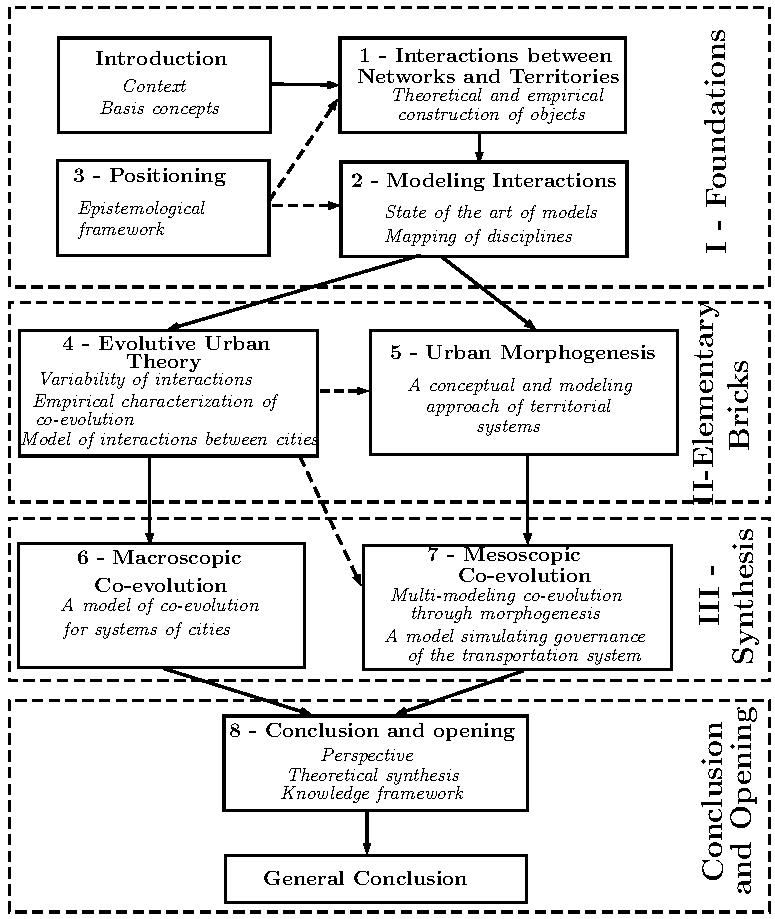
\includegraphics[width=\linewidth]{Figures/Theory/plan_en.pdf}
		}{
		  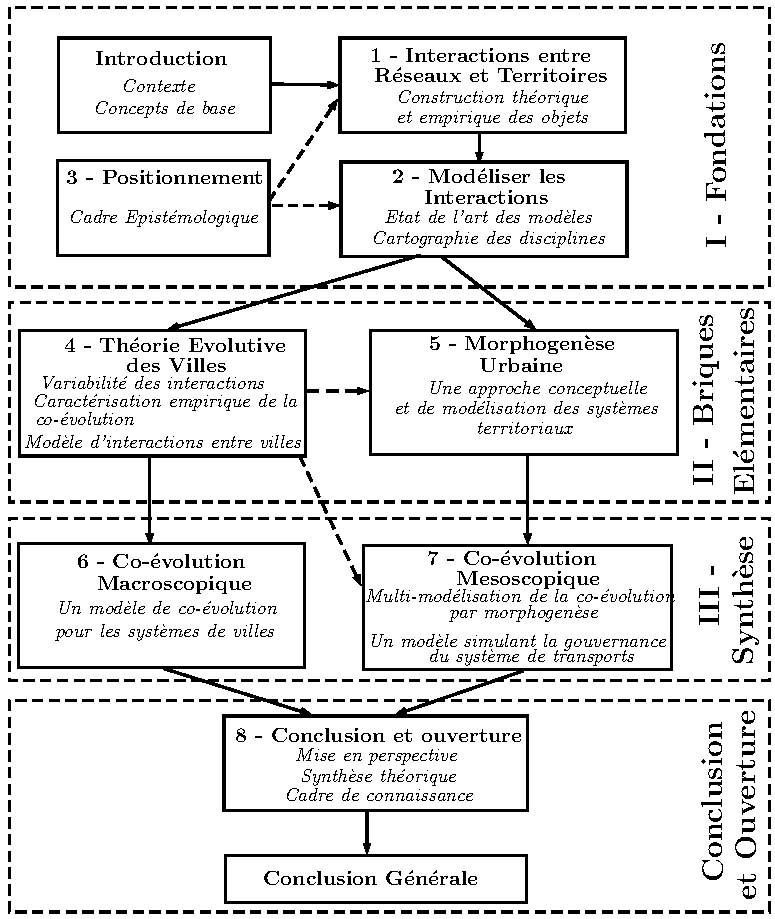
\includegraphics[width=\linewidth]{Figures/Theory/plan.pdf}
		}
		
		\medskip
		
		\framecaption{\textbf{General organisation of the memoire.} Full arrows give a direct dependency (logical chaining or extensions), dotted arrows an indirect dependency (reuse of data or methods).\label{frame:intro:organisation}}{\textbf{Organisation générale du mémoire.} Les flèches pleines donnent une dépendance directe (enchainement logique ou extensions), les flèches pointillées une dépendance indirecte (réutilisation de données ou de méthodes).\label{frame:intro:organisation}}
	\end{mdframed}
\end{figure}
%%%%%%%%%%%




%\paragraph{On linear reading}{Sur la lecture linéaire}

%%%%%%%
%% -- ON HOLD -- (depends on reflexive analysis - last appendix)


%\comment{expliquer notre position sur la difficulté d'une présentation linéaire, au delà de faire la synthèse. // bon bouquins y arrivent ? y réfléchir. la métaphore narrative intro/cl parties sera ce squelette linéaire. les deux approches sont compatibles.}


%\bpar{
%Research question and precise objects are deliberately fuzzy for now, as we postulate that the construction of a problematic can not be dissociated from the production of a corresponding theory. Reciprocally, it makes no sense to ask questions out of the blue, on objects that have been only partially or rapidly defined. Our preliminary question to enter the subject, that we can obtain from concrete cases such as our introducing anecdote or from preliminary literature review, is the following :
%}{
%Dans tous les cas, nous postulons que la construction d'une problématique ne peut être dissociée de la production d'une théorie correspondante. De manière réciproque, il n'y a aucun sens à poser des questions sorties de nulle part, sur des objets qui ont été seulement partiellement ou brièvement définis. Notre question préliminaire pour entrer dans le sujet, qu'on peut obtenir à partir de cas concrets comme l'anecdote introductive ou la revue de littérature préliminaire, est la suivante :
%}









\stars



